\documentclass[withoutpreface,bwprint]{cumcmthesis}
\usepackage{tikz}
\usetikzlibrary[arrows,patterns]
\usepackage{pgfplots}

\pgfplotsset{compat = 1.8}
\pgfplotsset{every axis label/.append style={font=\small}}
\pgfplotsset{every tick label/.append style={font=\small}}
\pgfplotsset{every legend label/.append style = {font = \small}}

\newcommand{\prb}{\times 10^5~\mathrm{kPa}}
\newcommand{\pre}{~\mathrm{kPa}}
\newcommand{\vol}{~\mathrm{mm^3}}
\newcommand{\are}{~\mathrm{mm^2}}
\newcommand{\len}{~\mathrm{mm}}
\newcommand{\tim}{~\mathrm{ms}}
\newcommand{\vel}{~\mathrm{ms^{-1}}}
\newcommand{\mas}{~\mathrm{mg}}
\newcommand{\den}{~\mathrm{mg~mm^{-3}}}
\newcommand{\flo}{~\mathrm{mm^3~ms^{-1}}}

\newcommand{\pres}{/\mathrm{kPa}}
\newcommand{\vols}{/\mathrm{mm^3}}
\newcommand{\ares}{/\mathrm{mm^2}}
\newcommand{\lens}{/\mathrm{mm}}
\newcommand{\tims}{/\mathrm{ms}}
\newcommand{\vels}{/\mathrm{ms^{-1}}}
\newcommand{\mass}{/\mathrm{mg}}
\newcommand{\dens}{/\mathrm{mg~mm^{-3}}}
\newcommand{\flos}{/\mathrm{mm^3~ms^{-1}}}
%\documentclass[withoutpreface,bwprint]{cumcmthesis} %去掉封面与编号页
\usepackage{listings}
\usepackage{xcolor}
\usepackage{lmodern}
% 配置代码高亮
\lstset{
	basicstyle          =   \sffamily,          % 基本代码风格
	keywordstyle        =   \bfseries,          % 关键字风格
	commentstyle        =   \rmfamily\itshape,  % 注释的风格,斜体
	stringstyle         =   \ttfamily,  % 字符串风格
	flexiblecolumns,                % 别问为什么,加上这个
	numbers             =   left,   % 行号的位置在左边
	showspaces          =   false,  % 是否显示空格,显示了有点乱,所以不现实了
	numberstyle         =   \zihao{-5}\ttfamily,    % 行号的样式,小五号,tt等宽字体
	showstringspaces    =   false,
	captionpos          =   t,      % 这段代码的名字所呈现的位置,t指的是top上面
	frame               =   lrtb,   % 显示边框
}
\lstdefinestyle{Python}{
	language        =   Python, % 语言选Python
	basicstyle      =   \zihao{-5}\ttfamily,
	numberstyle     =   \zihao{-5}\ttfamily,
	keywordstyle    =   \color{blue},
	keywordstyle    =   [2] \color{teal},
	stringstyle     =   \color{magenta},
	commentstyle    =   \color{red}\ttfamily,
	breaklines      =   true,   % 自动换行,建议不要写太长的行
	columns         =   fixed,  % 如果不加这一句,字间距就不固定,很丑,必须加
	basewidth       =   0.5em,
}

\title{高压油管的压力控制}
\tihao{A}
\baominghao{201901001042}
\schoolname{北京大学}
\membera{李婧宜}
\memberb{曹宇创}
\memberc{谭淞宸}
\supervisor{无}
\yearinput{2019}
\monthinput{09}
\dayinput{13}

\begin{document}

\maketitle
\begin{abstract}
	本文中我们先给出了每一题的基本分析和思路,再给出了它们的具体解题过程。

	对于问题一,我们假定高压油管内燃油压强均匀,高压油泵的流量符合题中注2所给公式。我们预先根据题目中给的弹性模量和压强的关系,用梯形法数值积分得到了在离散点上燃油密度和压强的对应关系,在后面程序使用时通过线性内插得到完整函数关系。我们先通过稳压近似方法,利用长时间内燃油流入质量等于流出质量给出单向阀开启时长的理论值;再通过将时间离散化,用数值模拟的方法给出压强精确演化规律,并对两种方法的结果进行了交叉验证。
	
	对于问题二,我们建立了一个考虑了油泵和喷油器工作原理的演化模型。我们预先利用凸轮的外轮廓形状计算了在给定转角下柱塞的抬升高度。再将燃油在喷油器内的行为近似为了两次扩散过程,并利用已知的针阀升程的变化,通过割线法求解了给定时间和油管压强下的喷油器流量。最后我们将油泵、油管和喷油器三个部件组合到一起,完成系统的模拟演化程序。我们定义关于目标压强的方均根偏差作为压强偏离的量度,得出了最优凸轮角速度为$\omega=0.0238\vel$。
	
	对于问题三,首先我们从上一问找出了压强波动的原因。联系实际情况确定了系统的哪些量可以进行调整。我们先对减压阀可连续调节的情况,通过定性半定量分析得出最优的控制方案应满足的条件,再通过数值模拟和参数调整得到具体的控制方案,该方案能够将压强的波动缩小接近100倍。然后又考虑了实际应用中可能对阀门控制有所限制,构造了另一种阀门操作频率很低的控制方案,能将压强波动缩小约4倍,并从理论上证明了在给定限制条件下该方案的最优性。
	
	在本文的最后,我们对上述建立的模型进行了评价,说明了它的合理性和可拓展性,同时指出了一些近似导致的模型的局限性。
\\
\keywords{高压油管\quad 数值模拟\quad 稳压控制}
\end{abstract}

\section{问题的表述与分析}
\subsection{引言}

高压油管(以下简称油管)被广泛应用于柴油机等燃油发动机中\cite{引言},燃油经过高压油泵(以下简称油泵)进入油管,再由喷口喷出。燃油的周期性进入与喷出会导致油管内压力的变化,直接影响其所匹配燃油机性能的稳定性和工作的可靠性。具体而言,管内压强的波动将导致排气温度不稳定,降低了催化剂的转换效率,使燃油机排放一致性下降。因此,减小管内压力的波动从而提升工作效率,是当前高压燃油系统亟需解决的技术难题。

本文中,所有长度均以 $\mathrm{mm}$ 为单位,所有质量均以 $\mathrm{mg}$ 为单位,所有时间均以 $\mathrm{ms}$ 为单位。由于压强的量纲为 $\mathrm{ML^{-1}T^{-2}}$,当使用上述三个基本力学量的单位时,压强的自然单位是 $\mathrm{kPa}$,因此本文中所有压强均以 $\mathrm{kPa}$ 为单位。

\subsection{问题 1}
\subsubsection{问题 1 的表述}

已知供油系统 1(以下简称系统 1,下同)的示意图为图 \ref{system1},由以下三部分组成:

\begin{figure}[!ht]
	\centering
	\begin{tikzpicture}
		\draw [very thick] 
		(-1.4, 0.8) -- (0.5, 0.8) -- (0.5, 0) -- 
		(10, 0) -- (10, -1) -- (9, -1) -- (9, -1.6) --
		(8.8, -2.0);
		\draw [very thick]
		(-1.4, 0.6) -- (0.3, 0.6) -- (0.3, 0) -- (0, 0) --
		(0, -1) -- (8.4, -1) -- (8.4, -1.6) -- 
		(8.6, -2.0);
		\draw (0.8, 0.3) [blue] node {\large A};
		\draw [->, red, thick] (-2.4, 0.7) -- (-1.6, 0.7);
		\draw (-2, 0.3) [blue] node {\large 高压油泵};
		\draw (5, -0.5) [blue] node {\large 高压油管};
		\draw (9.3, -1.3) [blue] node {\large B};
		\draw (7.7, -1.3) [blue] node {\large 喷油器};
		\draw [->, red, thick] (8.7, -2.2) -- (8.7, -3);
	\end{tikzpicture}
	\caption{系统 1 示意图}
	\label{system1}
\end{figure}

\begin{itemize}
	\item 单向阀 A:将油泵连接到油管,截面内径为 $1.4\len$;单向阀打开时向油管内供油,压强恒为 $1.6\prb$,且每打开一次后就要关闭 $10\tim$;
	\item 油管:内腔长度为 $500\len$,内直径为 $10\len$,初始压强为 $1\prb$;
	\item 喷油器 B:每秒工作 $10$ 次,每次工作时喷油时间为 $2.4\tim$,工作时向外喷油的速率如图 \ref{flow} 所示。
\end{itemize}

\begin{figure}[!ht]
	\centering
	\begin{tikzpicture}
		\begin{axis}[
		xlabel={时间$\tims$},
		ylabel={喷油速率$\flos$},
		width = 15cm,
		height = 5cm,
		ymin = 0,
		ymax = 25,
		xmin = 0,
		xmax = 2.6,
		xtick distance = 0.2
		]
		\addplot [blue] table {
			x y
			0 0
			0.2 20
			2.2 20
			2.4 0
		};
		\end{axis}
	\end{tikzpicture}
	\caption{喷油速率示意图}
	\label{flow}
\end{figure}

现有如下问题:

\begin{itemize}
	\item 单向阀开启时长(以下简称开启时长)为多少时,系统演化过程中油管内燃油压强关于目标压强 $1\prb$ 有最小的偏离?
	\item 开启时长为多少时,油管内燃油压强将在约 $2000\tim$、$5000\tim$ 和 $10000\tim$ 的调整过程后达到 $1.5\prb$?
	\item 达到 $1.5\prb$ 之后,开启时长为多少时,系统演化过程中油管内燃油压强关于目标压强 $1\prb$ 有最小的偏离?
\end{itemize}

\subsubsection{问题 1 的分析}
问题 1 的第 1 小问要求我们通过设置开启时长使得油管内燃油压强稳定在 $1\prb$。由喷油速率示意图,在喷油器的一个工作周期($100\tim$)内,喷油器喷出的油量为 $44\vol$,而油管的容积为 $3.93\times 10^4\vol$,可见油管中的油量变化在 $0.1\%$ 上下,由此我们得出两种解题思路:

\textbf{稳压近似方法}:即近似认为油管内燃油压强稳定在 $1\prb$ 时,其压强波动可以忽略不计。在一个工作周期内,喷油器喷出的流量已知;且在压强不变的近似下,单向阀流入的流速也已知。若要求压强稳定,必然有流入质量和流出质量相等,据此可以解出一个工作周期内单向阀应当开启的时间,进行等比例转换后即能得到单向阀每次开启的时间。

\textbf{数值模拟方法}:即不作近似,而是对系统的演化进行精确的数值模拟。在数值模拟中,我们采取较小的时间步长(如 $0.01\tim$),在每一步计算单向阀流入的流量和喷油器流出的流量,并根据出入流量计算油管内燃油的质量变化,进而得到更新后的油管内燃油的密度和压强,并计算其关于 $1\prb$ 的偏离大小。

通过数值模拟方法,我们可以验证我们通过稳压近似方法选取的开启时长是否是在精确模拟中使得压强偏离最小的开启时长。

对于问题 1 的第 2 小问,对于每一个给定的调整过程长度,我们可以通过数值模拟方法尝试一系列可能的开启时长,对于每一个开启时长计算调整过程过后油管内燃油压强关于目标压强的偏离,从而选取最优的开启时长。

对于问题 1 的第 3 小问,我们可以通过类似于第 1 小问的方法计算出对应于目标压强 $1.5\prb$ 的开启时长。
\subsection{问题 2}
\subsubsection{问题 2 的表述}
已知系统 2 的示意图为图 \ref{system2},由以下三部分组成:


\begin{figure}[!ht]
	\centering
	\begin{tikzpicture}
		% 轮廓线
		\draw [very thick] 
		(-2, 0.6) -- 
		(-2, 0) -- (-1.4, 0) -- (-1.4, -1.8) -- 
		(-2.8, -1.8) -- (-2.8, 0) -- (-2.2, 0) --
		(-2.2, 0.8) -- (0.5, 0.8) -- (0.5, 0) -- 
		(10, 0) -- (10, -1) -- (9, -1) -- (9, -1.6) --
		(8.8, -2.0);
		\draw [very thick]
		(-2, 0.6) -- (0.3, 0.6) -- (0.3, 0) -- (0, 0) --
		(0, -1) -- (8.4, -1) -- (8.4, -1.6) -- 
		(8.6, -2.0);
		\filldraw (-1.4, -1.2) rectangle (-2.8, -1.3);
		\draw [very thick] (-2.1, -1.3) -- (-2.1, -2.2);
		\draw [very thick] (-1.8, -2.2) -- (-2.4, -2.2);
		% 批注
		\draw (0.8, 0.3) [blue] node {\large A};
		\draw (-2.1, -0.4) [blue] node {\large 高压};
		\draw (-2.1, -0.9) [blue] node {\large 油泵};
		\draw (5, -0.5) [blue] node {\large 高压油管};
		\draw (9.3, -1.3) [blue] node {\large B};
		\draw (7.7, -1.3) [blue] node {\large 喷油器};
		% 箭头
		% \draw [->, red, thick] (-3, 0.7) -- (-2.2, 0.7);
		\draw [->, red, thick] (8.7, -2.2) -- (8.7, -3);
		% 针阀
		\draw [thick] (8.7, -0.8) -- (8.7, -1.2);
		\draw [very thick, xshift = -2.1cm, yshift = -3.1cm, domain=0:2*pi, samples=200, smooth] plot (xy polar cs:angle=\x r, radius={0.5+0.4*sin(\x r)});
		\filldraw (-2.1, -3) circle [radius = 0.05cm];
		\filldraw [fill=gray!50, draw=black, thick] (8.55, -1.2) rectangle (8.85, -1.8);
	\end{tikzpicture}
	\caption{系统 2 示意图}
	\label{system2}
\end{figure}

\begin{itemize}
	\item 单向阀 A:将油泵与油管连接,截面内径为 $1.4\len$;燃油来自油泵的柱塞腔出口,当柱塞腔内的压强大于油管内燃油压强时,柱塞腔与油管连接的单向阀开启,燃油进入油管内。柱塞上下运动由凸轮驱动,柱塞腔内径为 $5\len$,运动到上止点位置时,柱塞腔残余容积为 $20\vol$;柱塞运动到下止点时,压强为 $500\pre$ 的低压燃油会充满柱塞腔;
	\item 油管:内腔长度为 $500\len$,内直径为 $10\len$,初始压强为 $1\prb$;
	\item 喷油器 B:喷油器喷油器结构如图 4 所示,每秒工作 $10$ 次,喷油量由针阀控制。针阀直径为 $2.5\len$、密封座是半角为 $\pi/20$ 的圆锥,最下端喷孔的直径为 $1.4\len$。针阀升程为 $0$ 时,针阀关闭;针阀升程大于 $0$ 时,针阀开启,燃油向喷孔流动,通过喷孔喷出。
\end{itemize}

现有如下问题:
\begin{itemize}
	\item 凸轮的角速度为多少时,系统演化过程中油管内燃油压强关于目标压强 $1\prb$ 有最小的偏离?
\end{itemize}

\subsubsection{问题 2 的分析}

问题 2 相较于问题 1,需要考虑额外的两个问题:

\begin{enumerate}
	\item 由于系统 2 中油泵柱塞由凸轮驱动,我们首先需要将凸轮的边缘曲线转化为凸轮转过不同角度时柱塞的高度;
	\item 由于系统 2 中未给出喷油器 B 的流量,需要我们根据压强以及几何形状求解相应的流量。
\end{enumerate}

在此基础上,我们可以使用和问题 1 中相同的算法,对油泵和油管分别动态地更新压强和密度,实现对系统 2 的数值模拟。通过对不同的角速度下系统的演化进行模拟计算,我们可以得出使得关于目标压强 $1\prb$ 偏离最小的角速度。

\subsection{问题 3}
\subsubsection{问题 3 的表述}

已知系统 3 的示意图为图 \ref{system2},由以下三部分组成:

\begin{figure}[!ht]
	\centering
	\begin{tikzpicture}
		% 轮廓线
		\draw [very thick] 
		(-2, 0.6) -- 
		(-2, 0) -- (-1.4, 0) -- (-1.4, -1.8) -- 
		(-2.8, -1.8) -- (-2.8, 0) -- (-2.2, 0) --
		(-2.2, 0.8) -- (0.5, 0.8) -- (0.5, 0) -- 
		(10, 0) -- (10, -1) -- (9, -1) -- (9, -1.6) --
		(8.8, -2.0);
		\draw [very thick]
		(-2, 0.6) -- (0.3, 0.6) -- (0.3, 0) -- (0, 0) -- (0, -0.4) -- (-0.6, -0.4) -- (-0.6, -1);
		\draw [very thick] (-0.4, -1) -- (-0.4, -0.6) -- (0, -0.6) -- (0, -1) -- (4.4, -1) -- (4.4, -1.6) -- (4.6, -2.0);
		\draw [very thick] (4.8, -2.0) -- (5, -1.6) -- (5, -1) -- (7, -1) -- (8.4, -1) -- (8.4, -1.6) -- (8.6, -2.0);
		\filldraw (-1.4, -1.2) rectangle (-2.8, -1.3);
		\draw [very thick] (-2.1, -1.3) -- (-2.1, -2.2);
		\draw [very thick] (-1.8, -2.2) -- (-2.4, -2.2);
		% 批注
		\draw (0.8, 0.3) [blue] node {\large A};
		\draw (-2.1, -0.4) [blue] node {\large 高压};
		\draw (-2.1, -0.9) [blue] node {\large 油泵};
		\draw (5, -0.5) [blue] node {\large 高压油管};
		\draw (9.3, -1.3) [blue] node {\large B};
		\draw (7.7, -1.3) [blue] node {\large 喷油器};
		\draw (5.3, -1.3) [blue] node {\large C};
		\draw (3.7, -1.3) [blue] node {\large 喷油器};
		\draw (0.3, -0.5) [blue] node {\large D};
		\draw (0.3, -1.3) [blue] node {\large 减压阀};
		% 箭头
		\draw [->, red, thick] (-0.5, -1.2) -- (-0.5, -2);
		\draw [->, red, thick] (8.7, -2.2) -- (8.7, -3);
		\draw [->, red, thick] (4.7, -2.2) -- (4.7, -3);
		% 针阀 B
		\draw [thick] (8.7, -0.8) -- (8.7, -1.2);
		\filldraw [fill=gray!50, draw=black, thick] (8.55, -1.2) rectangle (8.85, -1.8);
		% 针阀 C
		\draw [thick] (4.7, -0.8) -- (4.7, -1.2);
		\filldraw [fill=gray!50, draw=black, thick] (4.55, -1.2) rectangle (4.85, -1.8);
		% 凸轮
		\draw [very thick, xshift = -2.1cm, yshift = -3.1cm, domain=0:2*pi, samples=200, smooth] plot (xy polar cs:angle=\x r, radius={0.5+0.4*sin(\x r)});
		\filldraw (-2.1, -3) circle [radius = 0.05cm];
	\end{tikzpicture}
	\caption{系统 3 示意图}
	\label{system3}
\end{figure}

\begin{itemize}
	\item 单向阀 A:与系统 2 中相同,并假设凸轮仍为匀速转动;
	\item 油管:与系统 2 中相同;
	\item 喷油器 B、C:结构与系统 2 中相同,考虑到实际应用\cite{保持频率不变},B 和 C 能够调节的只有二者喷油的时间间隔,而喷油频率保持不变;
	\item 单向减压阀 D(以下简称减压阀):打开减压阀时油管内的燃油可以回流到外部低压油路中,使得油管内的压强减小\cite{减压阀}。由于题目并没有明确说明减压阀是否可以连续控制,在本题中我们将按以下两种情况进行分类讨论:
	\begin{enumerate}
		\item 减压阀可以随时开启和关闭,不受任何限制;
		\item 减压阀每次开启后需要至少 $10\tim$ 的关闭时间,与问题 1 中类似。
	\end{enumerate}
\end{itemize}

现有如下问题:

\begin{itemize}
	\item 当减压阀不受限制时,凸轮的角速度为多少、B 和 C 的喷油时间间隔为多少、D 采取何种控制方案时,系统演化过程中油管内的压强关于目标压强 $1\prb$ 有最小的偏离?
	\item 当减压阀受到限制时,凸轮的角速度为多少、B 和 C 的喷油时间间隔为多少、D 采取何种控制方案时,系统演化过程中油管内的压强关于目标压强 $1\prb$ 有最小的偏离?
\end{itemize}

\subsubsection{问题 3 的分析}
理解此问题的关键在于找到压强波动的原因。由于具体分析需要用到问题2的结果,我们将在后文根据问题 2 的结果进行详细分析,在此不再赘述。

\newpage
\section{模型的建立与求解}
\subsection{符号说明}

现将本文使用的主要符号列于下表:

\begin{table}[!ht]
    \begin{minipage}{\textwidth}
        \begin{minipage}[t]{0.5\textwidth}
        \centering
        \caption{符号说明}
        \begin{tabular}{cc}
        \toprule
        符号             & 物理量           \\
		\midrule
		$P_0$          & 大气压            \\
        $V_1$          & 油泵体积          \\
		$m_1$          & 油泵中燃油质量     \\
		$\rho_1$       & 油泵中燃油密度       \\
        $P_1$          & 油泵中燃油压强          \\
        $V_2$          & 油管体积          \\
		$m_2$          & 油管中燃油质量     \\
        $\rho_2$       & 油管中燃油密度       \\
        $P_2$          & 油管中燃油压强          \\
		$P_2^*$        & 油管中燃油的目标压强     \\
		$\rho_3$       & 喷油器缓冲区中燃油密度   \\
		$P_3$          & 喷油器缓冲区中燃油压强   \\
        $\theta$       & 凸轮各点极角        \\
        $\alpha$       & 凸轮极轴方位角       \\
        $h$            & 凸轮最高点高度       \\
        $\omega$       & 凸轮角速度         \\
        $\gamma$       & 圆锥半角          \\
		$z$            & 针阀高度          \\ 
		\bottomrule
        \end{tabular}
        \end{minipage}
        \begin{minipage}[t]{0.5\textwidth}
        \centering
        \caption{符号说明(续)}
        \begin{tabular}{cc}
        \toprule
        符号             & 物理量           \\
        \midrule
        $d_A$          & 单向阀 A 截面直径       \\
        $S_A$          & 单向阀 A 截面面积       \\
        $Q_A$          & 单向阀 A 截面流量       \\
        $\tau_A^+$     & 单向阀 A 的开启时长     \\
        $\tau_A^-$     & 单向阀 A 的关闭时长     \\
        $\tau_A$       & 供油周期       \\
        $d_B$          & 喷油器 B 截面直径       \\
        $S_B$          & 喷油器 B 截面面积       \\
        $S_B'$          & 喷油器 B 针阀处等效截面面积      \\
		$Q_B$          & 喷油器 B 截面流量      \\
		$\phi_B$         & 喷油器 B 相位  \\
        $\tau_B$       & 喷油周期       \\
        $\tau_B'$       & 喷油等效周期       \\
		$\tau_B^{(A)}$       & 喷油周期内 A 的总开启时长  \\
		$\tau_I$     &       调整过程时长 \\
		$\Delta t$ & 模拟步长 \\
		$D$            & 油管中燃油压强的均方根偏差 \\
		$D_{\max}$    & 油管中燃油压强的最大偏差  \\
		$E$     & 油管中燃油压强的极差 \\
		\bottomrule
        \end{tabular}
        \end{minipage}
    \end{minipage}
\end{table}



\newpage
\subsection{问题一的求解}

\subsubsection{数据预处理}

为考察系统在不同压强下的行为,首先要建立压强和燃油密度的函数关系。但题目中只给出了压强与弹性模量的关系,因此我们通过数据预处理的步骤将它转化为所需要的数据形式。

由题意,燃油的压强变化量与密度变化量成正比,比例系数为 $E/\rho$,且已知标准态 $P^*=1\prb$ 对应着 $\rho^* = 0.850\den$。据此我们可以列出如下的微分方程:

$$
\frac{\mathrm dP}{\mathrm d\rho}=\frac{E}{\rho}
$$

由于题目中将 $E$ 表示为 $P$ 的函数,我们进行移项并积分,得到:

$$
\int_{P^*}^{P}\frac{\mathrm dP'}{E(P')}=\int_{\rho^*}^{\rho}\frac{\mathrm d\rho'}{\rho'}=\ln\rho-\ln\rho^*
$$

但对于函数 $E(P)$ 我们只知道有限个点的函数值,因此左方的积分必须通过数值积分的方法计算,为此我们首先选取上限 $P = 1.005\prb$,将左方的积分近似表示为 $(E(P^*)^{-1}+E(P)^{-1})(P-P^*)/2$,而这两点处的函数值均已知,进而右方的 $\rho$ 可以从上式中解出。依此类推,每次积分 $500\pre$ 的区间,逐次迭代得到若干个 $\rho$ 的函数值直至 $2\prb$,再向反方向逐次迭代直至 $0$,即得到所需的函数关系。

\subsubsection{基于平均化近似的开启时长计算}

首先假设油管内燃油压强近似保持在 $P_2=P_2^*=1\prb$,因而油管内燃油密度 $\rho_2$ 为常数。在一个喷油周期 $\tau_B$ 内,从喷油器流出的燃油质量 $\Delta m$ 由流量与密度给出:

$$
\Delta m=\int_0^{\tau_B}Q_B\rho_2\mathrm dt=37.4\mas
$$

这些质量应当由从单向阀流入的燃油补充,因此在一个 $\tau_B$ 内,单向阀总开启时长 $\tau_B^{(A)}$ 应当由损失的质量和补充燃油质量的速度决定:

$$
\begin{aligned}
\tau_B^{(A)}&=\frac{\Delta m}{Q_A\rho_1}\\
&=\frac{\Delta m}{\rho_1CS_A\sqrt{2(P_1-P_2)/\rho_1}}\\
&=2.80\tim
\end{aligned}
$$

若我们考虑系统进行较长时间的演化,则 $\tau_B^{(A)}$ 占 $\tau_B$ 的比例,应该与单向阀开启时长 $\tau_A^+$ 占供油周期 $\tau_A$ 的比例相同。因此,$\tau_A^+$ 与 $\tau_A$ 应该满足如下比例式:

$$
\frac{\tau_A^+}{\tau_A}=\frac{\tau_B^{(A)}}{\tau_B}
$$

代入已知数据,可以求出 $\tau_A^+=0.288\tim$。

\subsubsection{系统 1 的数值模拟}

在数值模拟中,我们设定初始条件为油管内燃油压强 $P_2=1\prb$,且时间零点恰好位于供油周期的开始,但可以位于喷油周期中的任意一点,该点处相位时间为 $\phi_B$。经多次模拟发现,$\phi_B$ 对系统演化的影响在演化时间 $>1000\tim$ 时可以忽略不计,因此本题中取为 $0$。

系统的演化算法可以用如下关系表示,其中左箭头「$\leftarrow$」是程序设计中的赋值等号:

$$
\begin{aligned}
    Q_A &\leftarrow Q_A(t)\\
    Q_B &\leftarrow Q_B(t)\\
    m_2 &\leftarrow m_2 + Q_A \times \rho_1 \times \Delta t - Q_B \times \rho_2 \times \Delta t\\
    \rho_2 &\leftarrow m_2 / V_2\\
    P_2 &\leftarrow P(\rho_2)\\
\end{aligned}
$$

例如,当取单向阀开启时长 $\tau_A^+=0.288\tim$ 时,系统在第一个喷油周期内的压强变化如图\ref{firstperiodPt} 所示:

\begin{figure}[!ht]
	\centering
	\begin{tikzpicture}
	\begin{axis} [
		width = 10cm,
		height = 5cm,
		xlabel = {$t\tims$},
		ylabel = {$P_2-P_2^*\pres$},
		xmin = 0, 
		xmax = 100,
		ymin = -2400,
		ymax = 400,
		ytick distance = 400,
	]
	\addplot table [
		x=t, 
		y=P, 
		mark=none, 
		smooth] {../1/P-t.dat};
	\end{axis}
	\end{tikzpicture}
	\caption{$\tau_A^+=0.288\tim$ 时,第一个喷油周期内$P_2$ 与 $t$ 的关系}
	\label{firstperiodPt}
\end{figure}

为了定量刻画 $P_2$ 关于目标压强 $P_2^*$ 的平均偏离,我们将系统进行 $N$ 个喷油周期的演化,获得各个时刻的 $P_2(t)$ 后,定义关于 $P_2*$ 的均方根偏差 $D$ 作为 $P_2(t)$ 的泛函:

$$
D[P_2(t)]=\sqrt{\frac1{N\tau_B}\int_0^{N\tau_B}
\left[P_2(t)-P_2^*\right]^2\mathrm dt}
$$

由于从单向阀流入的燃油量随 $\tau_A^+$ 单调递增,对于给定的 $P_2^*$,$D$ 在 $\tau_A^+$ 不断增大时一定是先减小后增大的。因此,给定一系列 $\tau_A^+$,计算它们对应的 $D$,就可以从曲线的最低点处找出使得 $D$ 最小的开启时长。图 \ref{Dtau} 给出了演化不同喷油周期数时,$D$ 与 $\tau_A^+$ 的关系:

\begin{figure}[!ht]
	\centering
	\begin{tikzpicture}[scale=1]
	\begin{axis}[
		width = 15cm,
		height = 10cm,
		xlabel={$\tau_A^+\tims$},
		ylabel={$D\pres$},
		xmin=0.280,
		xmax=0.300,
		ymin=600,
		ymax=1800,
		legend style={nodes={transform shape},at={(0.4,1)}},
		yticklabel style={
			/pgf/number format/fixed,
			/pgf/number format/precision=0,
			/pgf/number format/fixed zerofill
			},
		xticklabel style={
			/pgf/number format/fixed,
			/pgf/number format/precision=3,
			/pgf/number format/fixed zerofill,}
		]
	
	\addplot table [x=tauA, y=D, smooth] {../1/D-tauA20.dat};
	\addplot table [x=tauA, y=D, smooth] {../1/D-tauA40.dat};
	\addplot table [x=tauA, y=D, smooth] {../1/D-tauA60.dat};
	\addplot table [x=tauA, y=D, smooth] {../1/D-tauA80.dat};
	\addplot table [x=tauA, y=D, smooth] {../1/D-tauA100.dat};
	\addlegendentry{$N=20$}
	\addlegendentry{$N=40$}
	\addlegendentry{$N=60$}
	\addlegendentry{$N=80$}
	\addlegendentry{$N=100$}
	\end{axis}
	\end{tikzpicture}
	\caption{模拟不同喷油周期数时,$D$ 与 $\tau_A^+$ 的关系}
	\label{Dtau}
\end{figure}

在图 \ref{Dtau} 中,为什么演化不同喷油周期数时,最优的开启时长不同呢?这是因为,图 \ref{firstperiodPt} 中的 $P_2(t)$ 关系表明,$P_2$ 在大多数时间中对 $P_2^*$ 产生了负偏离,因此 $N$ 较小时,最优的 $\tau_A^+$ 较长(因而流入的燃油量较多)的方案具有优势;但 $N$ 较大时,只有流入质量和流出质量相等的方案才能在长期保持不偏离 $1\prb$,因此最优的 $\tau_A^+$ 较长。我们使用几个具有代表性的 $N$ 得到的最优的 $\tau_A^+$ 如图 \ref{tauN} 所示:

\begin{figure}
	\centering
	\begin{tikzpicture}
	\begin{axis}[
	yticklabel style={
		/pgf/number format/fixed,
		/pgf/number format/precision=3,
		},
	xticklabel style={
		/pgf/number format/fixed,
		/pgf/number format/precision=3,
		},
	width=15cm,
	height=7cm,
	grid=major, 
	grid style={dashed,gray!30},
	xlabel=$N$,
	ylabel=$\tau_A^+\tims$,
	xmode = log,
	]
	\addplot table[x=N, y=tau] {../1/tau-N.dat};
	\end{axis}
	\end{tikzpicture}
	\caption{最优的 $\tau_A^+$ 随 $N$ 的收敛性}
	\label{tauN}
\end{figure}

从这里我们可以得到两点结论:

\begin{itemize}
	\item 当 $N\to\infty$ 时,数值模拟得到的最优 $\tau_A^+$ 就是通过稳压近似得到的最优 $\tau_A^+$,这表明稳压近似能够较好地描述这一系统;
	\item 当 $N>100$ 时,这一结果接近于收敛,说明模拟 $100$ 个以上的喷油周期已经足以消除系统的任何暂态效应带来的影响。
\end{itemize}
\subsubsection{压力调整过程的模拟}
我们可以通过与第一小问中相同的方法,来近似计算令油管内燃油压强 $P_2$ 稳定在新的目标压强 $P_2^*=1.5\prb$ 所需要的单向阀开启时长 $\tau_A$,结果为 $\tau_A^+ = 0.752\tim$。根据第一小问中的结论,这一结果就是在当演化的喷油周期数 $N$ 趋于 $+\infty$ 时,使 $P_2$ 关于 $P_2^*$ 的均方根偏差 $D$ 最小的开启时长。

接下来我们考虑分别在调整过程时长 $t_I=2000, 5000, 10000\tim$ 的调整过程中应该令 $\tau_A^+$ 为多大。由于这一过程中 $P_2$ 发生了显著的变化,不能近似认为压强不变,因此难于解析求解。我们仍采用数值模拟的方法,通过扫描一个大致含有最优 $\tau_A^+$ 的时间范围来确定最优的 $\tau_A^+$。模拟分为两步:

\begin{enumerate}
	\item 调整过程中,将 $\tau_A^+$ 设定为我们试探的值,模拟至调整过程结束;
	\item 调整过程结束后,令 $\tau_A^+=0.752\tim$,继续模拟 $100$ 喷油周期,并以其为范围计算 $D$。
\end{enumerate}

计算结果如图 \ref{adjustment} 所示:

\begin{figure}[!ht]
	\centering
	\begin{tikzpicture}
		\begin{axis}[
			width = 5.5cm,
			height = 4cm,
			title = {$\tau_I=2000\tim$},
			label style={font=\large},
			tick label style={font=\large},
			xlabel={$\tau_A^+\tims$},
			ylabel={$D\pres$},
			ymin = 847,
			ymax = 850,
			xmin = 0.905,
			xmax = 0.935,
			xticklabel style={
				/pgf/number format/fixed,
				/pgf/number format/precision=3,
				/pgf/number format/fixed zerofill,},
		]
		\addplot table [x=tauA, y=D, smooth] {../1/adjustment_in_2000.dat};
		\end{axis}
	\end{tikzpicture}
	\hspace{-0.3cm}
	\begin{tikzpicture}
		\begin{axis}[
			width = 5.5cm,
			height = 4cm,
			title = {$\tau_I=5000\tim$},
			label style={font=\large},
			tick label style={font=\large},
			xlabel={$\tau_A^+\tims$},
			ymin = 847,
			ymax = 850,
			xmin = 0.745,
			xmax = 0.775,
			xticklabel style={
				/pgf/number format/fixed,
				/pgf/number format/precision=3,
				/pgf/number format/fixed zerofill,},
			yticklabel style={
				% font = \tiny,
				color = white,
			},
		]
		\addplot table [x=tauA, y=D, smooth] {../1/adjustment_in_5000.dat};
		\end{axis}
	\end{tikzpicture}
	\hspace{-0.3cm}
	\begin{tikzpicture}
		\begin{axis}[
			width = 5.5cm,
			height = 4cm,
			title = {$\tau_I=10000\tim$},
			label style={font=\large},
			tick label style={font=\large},
			xlabel={$\tau_A^+\tims$},
			ymin = 847,
			ymax = 850,
			xmin = 0.735,
			xmax = 0.765,
			xticklabel style={
				/pgf/number format/fixed,
				/pgf/number format/precision=3,
				/pgf/number format/fixed zerofill,},
			yticklabel style={
				% font = \tiny,
				color = white,
			},
		]
		\addplot table [x=tauA, y=D, smooth] {../1/adjustment_in_10000.dat};
		\end{axis}
	\end{tikzpicture}
	\caption{不同 $t_I$ 下 $D$ 与 $\tau_A^+$ 的关系}
	\label{adjustment}
\end{figure}

由此可见,$t_I$分别为 $2000, 5000, 10000\tim$ 时,最佳的 $\tau_A^+$ 分别为 $0.919$、$0.759$ 和 $0.756\tim$。
\subsection{问题二}
\subsubsection{数据预处理}
由题意,油泵通过柱塞实现泵油,柱塞由凸轮驱动上下运动,且已知凸轮边缘曲线与角度的关系,因此首先要将凸轮边缘曲线转化为柱塞的高度。

当凸轮极轴的转角为 $\alpha$ 时,凸轮上极角 $\theta$ 的方向对应的方位角为 $\alpha + \theta$。因此,我们可以选取一系列转角的数据点 $\alpha_i$,在每个数据点处遍历所有的极角 $\theta_j$,计算对应极径的高度并取最大值,作为柱塞的高度:

$$
h(\alpha_i)=\max_j(r_j\times \sin(\alpha_i+\theta_j))
$$

再对上述数据点处的高度 $h$ 进行线性内插即得到函数 $h(\alpha)$。
\subsubsection{锥形喷油器流速的求解\cite{锥形喷油嘴}}

题目中未给出喷油器的流速,因此需要利用密封座的几何参数进行求解。根据已知信息可以大致画出喷油器(为清楚展示,圆锥半角 $\gamma$ 有所夸大,图中 $d_I$ 为针阀截面直径,$l_1,l_2$ 为针阀边缘到锥面垂线及其反向延长线):

\begin{figure}[!ht]
	\centering
	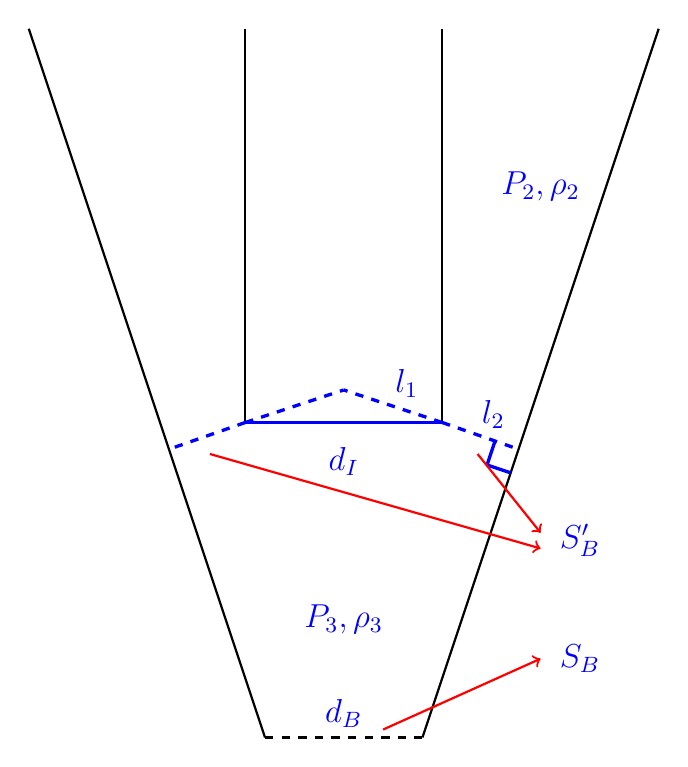
\begin{tikzpicture}
	  % 圆锥
	  \draw[dashed, very thick] (-1, 0) -- (1, 0);
	  \draw[thick] (-1, 0) -- (-4, 9);
	  \draw[thick] (1, 0) -- (4, 9);
	  % 针阀
	  \draw[thick] (-1.25, 9) -- (-1.25, 4.0);
	  \draw[blue, very thick] (-1.25, 4) -- (1.25, 4.0);
	  \draw[thick] (1.25, 9) -- (1.25, 4.0);
	  % 垂足
	  \draw[dashed, blue, very thick] (1.25, 4) -- (2.22, 3.66);
	  \draw[dashed, blue, very thick] (1.25, 4) -- (0, 4.413);
	  \draw[blue, very thick] (1.92, 3.76) -- (1.82, 3.46);
	  \draw[blue, very thick] (2.12, 3.36) -- (1.82, 3.46);
	  \draw[dashed, blue, very thick] (-1.25, 4) -- (0, 4.413);
	  \draw[dashed, blue, very thick] (-1.25, 4) -- (-2.22, 3.66);
	  % 说明文字
	  \draw (0, 0.3) [blue] node {\large $d_B$};
	  \draw[->, red, thick] (0.5, 0.1) -- (2.5, 1);
	  \draw (3, 1) [blue] node {\large $S_B$};
	  \draw[->, red, thick] (1.7, 3.6) -- (2.5, 2.6);
	  \draw[->, red, thick] (-1.7, 3.6) -- (2.5, 2.4);
	  \draw (3, 2.5) [blue] node {\large $S_B'$};
	  \draw (0, 1.5) [blue] node {\large $P_3,\rho_3$};
	  \draw (0, 3.5) [blue] node {\large $d_I$};
	  \draw (2.5, 7) [blue] node {\large $P_2,\rho_2$};
	  \draw (1.9, 4.1) [blue] node {\large $l_2$};
	  \draw (0.8, 4.5) [blue] node {\large $l_1$};
	\end{tikzpicture}
	\caption{喷油器示意图}
\end{figure}

由此看出,在喷油的过程中,针阀以下的部分形成了一个较大的空间,其体积至少为

$$
\frac{\pi}{24}\cot\gamma\times\left(d_I^3-d_B^3\right)\approx 10\vol
$$

而该部分体积与上下均有隔离,因此喷油过程可以用两次扩散过程进行近似。到达稳态时,两次扩散的流速相同,由此对喷油器可以列出以下方程:

$$
\begin{aligned}
Q_B=S_B'\sqrt{\frac{2(P_2-P_3)}{\rho_2}}=S_B\sqrt{\frac{2(P_3-P_0)}{\rho_3}}
\end{aligned}
$$

其中等效面积 $S_B'$ 的物理意义是从油管扩散到缓冲区时,所经过的最小截面面积,即针阀边缘到锥面的环形垂面的面积。计算公式为:

$$
\frac{1}{2}\pi{}(d_I+2l_2\cos{\gamma})(l_1+l_2)-\frac{1}{2}\pi d_Il_1 = \pi^2(z^2\sin{\gamma}^2\cos{\gamma}+d_Iz\sin{\gamma})
$$

通过该方程可以求出给定压强 $P_2$ 和给定针阀升程 $z$ 下的流量 $Q_B$。

\subsubsection{系统 2 的数值模拟}

在数值模拟中,我们设定初始条件为 $P_2=1\prb$,且时间零点恰好位于供油周期的开始(即凸轮高度下降到最低点),但可以位于喷油周期中的任意一点,该点处相位时间为 $\phi_B$。

系统的演化算法可以用如下关系表示:

$$
\begin{aligned}
	h &\leftarrow h(\alpha)\\
	Q_A &\leftarrow Q_A(t)\\
    Q_B &\leftarrow Q_B(t)\\
    m_1 &\leftarrow m_1 - Q_A \times \rho_1 \times \mathrm \Delta t\\
    m_2 &\leftarrow m_2 + Q_A \times \rho_1 \times \mathrm \Delta t - Q_B \times \rho_2 \times \Delta t\\
    \rho_1 &\leftarrow m_1 / V_1\\
    \rho_2 &\leftarrow m_2 / V_2\\
    P_1 &\leftarrow P(\rho_1)\\
    P_2 &\leftarrow P(\rho_2)\\
	\alpha &\leftarrow \alpha + \omega \times \Delta t\\
\end{aligned}
$$

我们仍以均方根误差 $D$ 为判据,计算不同角速度 $\omega$ 下,演化 $N=100$ 个喷油周期内的 $D$。由于从油泵流入的燃油量随 $\omega$ 单调递增,根据与系统 1 的数值模拟中相同的讨论,存在唯一的最优 $\omega$ 使得 $D$ 达到最小。图 \ref{Domega} 给出了一定范围内 $D$ 与 $\omega$ 的关系:

\begin{figure}[!ht]
	\centering
	\begin{tikzpicture}
	\begin{axis}[
		% axis lines=middle,
		% axis line style={->},
		% x label style={at={(axis description cs:0.5,-0.1)},anchor=north},
		% y label style={at={(axis description cs:-0.1,.5)},rotate=90,anchor=south},
		scaled ticks = false,
		width = 10cm,
		height = 5cm,
		xlabel={$\omega/\vel$},
		ylabel={$D/\pre$},
		ytick distance = 200,
		ymin = 1000,
		ymax = 2000,
		xmin = 0.0234,
		xmax = 0.0244,
		xtick distance = 0.0002,
		xticklabel style={
			/pgf/number format/fixed,
			/pgf/number format/precision=4,
			/pgf/number format/fixed zerofill}
	]
	\addplot table [x=omega, y=D, smooth] {../2/D-omega.dat};
	\end{axis}
	\end{tikzpicture}
	\caption{不同角速度下关于目标压强的均方根偏离}
	\label{Domega}
\end{figure}

由此可见 $\omega=0.0238\vel$ 为最优的角速度。此时油泵中燃油质量 $m_1$ 和油管中燃油压强 $P_2$ 随时间变化如图 \ref{allt} 所示:

\begin{figure}[!ht]
	\centering
	\begin{tikzpicture}
		\begin{axis}[
			name = first plot,
			xticklabel style = {
				color = white,
			},
			ylabel = {$m_1\mass$},
			xmin = 0,
			xmax = 1000,
			ymin = 10,
			ymax = 110,
			width = 15cm,
			height = 5cm,
		]
		\addplot table [x=t, y=m1, mark=none, smooth] {../2/m1-t.dat};
		\end{axis}
		\begin{axis}[
			name = second plot,
			at={(first plot.below south west)},
			yshift = 0cm,
			anchor = north west,
			xlabel = {$t\tim$},
			ylabel = {$P_2-P_2^*\pres$},
			xmin = 0,
			xmax = 1000,
			ymin = -2500,
			ymax = 2800,
			ytick distance = 1000,
			width = 15cm,
			height = 5cm,
		]
		\addplot table [x=t, y=P, mark=none, smooth] {../2/P-t.dat};
		\end{axis}
		\draw [->, red, thick] (3, -1.1) -- (1.5, -1.3);
		\draw [->, red, thick] (3.5, -1.4) -- (2.8, -2.3);
		\draw (3.5, -1.1) [blue] node {\large 喷油};
		\draw [->, red, thick] (1.5, -3.0) -- (0.7, -2.7);
		\draw (2.0, -3.0) [blue] node {\large 供油};
		% \draw [dashed, thick] (1, -4) -- (1, 3.4);
		% \begin{axis}[
		% 	name = third plot,
		% 	at={(second plot.below south west)},
		% 	yshift = 0cm,
		% 	anchor=north west,
		% 	xlabel={$t\tims$},
		% 	ylabel={$Q_A\flos$},
		% 	xmin = 0,
		% 	xmax = 1000,
		% 	width = 15cm,
		% 	height = 5cm,
		% ]
		% \addplot table [x=t, y=QA, mark=none, smooth] {../2/QA-t.dat};
		% \end{axis}
	\end{tikzpicture}
	\caption{$\omega=0.0238\vel$ 时前 $10$ 个喷油周期内 $m_1,P_2$ 和 $t$ 的关系}
	\label{allt}
\end{figure}

图 \ref{allt} 揭示了压强波动的原因。泵油时,$m_1$ 下降,$P_2$ 上升,其斜率较为平缓;而喷油时,$P_2$ 下降,其斜率较为陡峭。泵油和喷油时间不同,斜率也不同,导致油管内的燃油在某一些时间段过度累积,在另一些时间段过度消耗。即使选取了最优的 $\omega$,也仅能将 $D$ 降到 $1044\pre$ 左右。

\subsection{问题 3}
\subsubsection{减压阀连续控制情况:定性分析}

在问题 2 中我们看到,油管中燃油压强 $P_2$ 波动是由于喷油和泵油的时间不一致造成的。如果能在喷油的同时泵油,就能使得两者的效应相互抵消,压强波动变小。我们作如下约定:

\begin{itemize}
	\item 单位时间从油泵流入的燃油质量随时间的变化曲线称为「泵油曲线」;
	\item 单位时间从 B、C 两个喷油器流出的燃油质量随时间的变化曲线称为「喷油曲线」;
	\item 单位时间从单向阀流入的燃油质量减去从减压阀流出的燃油质量随时间的变化曲线称为「供油曲线」。
\end{itemize}

我们的目的在于使供油曲线和喷油曲线尽量重合,使得油管中尽量不产生燃油的积累或损失。在最理想的情况下,供油曲线和喷油曲线完全重合,此时油管中燃油质量 $m_2$ 不变,因而 $P_2$ 也保持不变。

通过减压阀的连续控制,可以随时开启减压阀来抵消油泵的供油,从而将供油曲线向下调整。例如,在喷油器关闭情况下,油泵却向油管内泵油,此时若 $P_2>1\prb$ 则开启减压阀,反之则关闭减压阀,可以保证其准确维持在目标压强 $P_2^*$ 附近(即供油曲线向下调整至 $0$)。当然,测量压强并实时反馈在应用中无法实现,这里仅通过该方法寻找控制策略;一旦找到策略,应用时只需按照预设时间开关减压阀即可,不再需要测量和反馈。

上述调节成立的条件是减压阀的流出率大于油泵的流入率。当$\omega$ 超过一定限度时时,打开减压阀时油管内压强仍然上升,调节功能失效;因此 $\omega$ 有上限值。

为了长时间的精确调节,供油周期 $\tau_A=2\pi/\omega$ 和喷油周期 $\tau_B$ 应当是简单整数比的关系。喷油的速率较大且比较恒定,为了使供油曲线贴近喷油曲线,$\tau_A$ 应该较小,合理的假设是 $\tau_A=\tau_B/M$,$M$ 为整数。在此基础上,为了使得 $\omega$ 较大,喷油器 B 和 C 应该交替喷油,这等效于 $\tau_B'=50\tim$ 的喷油周期。以下我们用 $Q_B$ 统一指代两个喷油器的流量。

我们以 $M=3$ 的情况为例,将上述分析直观展现在图 \ref{sketch31} 中。上图为泵油曲线,中图为供油曲线,下图为喷油曲线。减压阀将泵油曲线调节为供油曲线,使其贴近于喷油曲线。并且,为了使得流入燃油质量等于流出燃油质量,阴影部分应该面积相等。

\begin{figure}[!ht]
	\centering
	\begin{tikzpicture}
		\begin{axis}[
			name = first plot,
			xticklabel style = {
				color = white,
			},
			ylabel={$\mathrm dm/\mathrm dt ~(\mathrm{a. u.})$},
			xmin = 0,
			xmax = 1000,
			ymin = 0,
			ymax = 100,
			width = 15cm,
			height = 5cm,
			xtick=\empty,
			ytick=\empty,
		]
		\draw (50, 80) node {泵油曲线};
		\draw[thick] (0,10) -- (6.25,10);
		\draw[domain=6.25:18.75] plot(\x,{-1.408*(\x-12.5)^2+65});
		\draw[thick] (18.75,10) -- (31.25,10);
		\draw[domain=31.25:43.75] plot(\x,{-1.408*(\x-37.5)^2+65});
		\draw[thick] (43.75,10) -- (56.25,10);
		\draw[domain=56.25:68.75] plot(\x,{-1.408*(\x-62.5)^2+65});
		\draw[thick] (68.75,10) -- (81.25,10);
		\draw[domain=81.25:93.75] plot(\x,{-1.408*(\x-87.5)^2+65});
		\draw[thick] (93.75,10) -- (100,10);
		\end{axis}

		\begin{axis}[
			name = second plot,
			at={(first plot.below south west)},
			yshift = 0cm,
			anchor = north west,
			xticklabel style = {
				color = white,
			xtick=\empty,
			ytick=\empty,
			},
			ylabel={$\mathrm dm/\mathrm dt ~(\mathrm{a. u.})$},
			xmin = 0,
			xmax = 1000,
			ymin = 0,
			ymax = 100,
			%ytick distance = 400,
			width = 15cm,
			height = 5cm,
		]
		\draw (50, 80) node {供油曲线};
		\draw[thick] (0,10) -- (10.5,10);
		\draw[thick] (14.5,10) -- (85.5,10);
		\draw[thick] (89.5,10) -- (100,10);
		\draw[dashed,domain=6.25:18.75] plot(\x,{-1.408*(\x-12.5)^2+65});
		%\draw[thick] (18.75,10) -- (31.25,10);
		\draw[dashed,domain=31.25:43.75] plot(\x,{-1.408*(\x-37.5)^2+65});
		%\draw[thick] (43.75,10) -- (56.25,10);
		\draw[dashed,domain=56.25:68.75] plot(\x,{-1.408*(\x-62.5)^2+65});
		%\draw[thick] (68.75,10) -- (81.25,10);
		\draw[dashed,domain=81.25:93.75] plot(\x,{-1.408*(\x-87.5)^2+65});
		%\draw[thick] (93.75,10) -- (100,10);
		\draw[pattern=north west lines] (10.5,10) -- (10.5,59.368) plot [domain=10.5:14.5,smooth] (\x,{-1.408*(\x-12.5)^2+65})  -- (14.5,10) -- (10.5,10);
		%\draw[pattern=north west lines] (35.5,10) -- (35.5,59.368) plot [domain=35.5:39.5,smooth] (\x,{-1.408*(\x-37.5)^2+65})  -- (39.5,10) -- (35.5,10);
		%\draw[pattern=north west lines] (60.5,10) -- (60.5,59.368) plot [domain=60.5:64.5,smooth] (\x,{-1.408*(\x-62.5)^2+65})  -- (64.5,10) -- (60.5,10);
		\draw[pattern=north west lines] (85.5,10) -- (85.5,59.368) plot [domain=85.5:89.5,smooth] (\x,{-1.408*(\x-87.5)^2+65})  -- (89.5,10) -- (85.5,10);
		\end{axis}

		\begin{axis}[
			name = third plot,
			at={(second plot.below south west)},
			yshift = 0cm,
			anchor=north west,
			xlabel={$t~(\mathrm{a. u.})$},
			ylabel={$\mathrm dm/\mathrm dt ~(\mathrm{a. u.})$},
			xmin = 0,
			xmax = 1000,
			ymin=0,
			ymax=100,
			width = 15cm,
			height = 5cm,
			xtick=\empty,
			ytick=\empty,
		]
		\draw (50, 80) node {喷油曲线};
		\draw[thick] (0,10) -- (11.5,10);
		\draw[thick] (13.5,10) -- (86.5,10);
		%\draw[thick] (38.5,10) -- (61.5,10);
		%\draw[thick] (63.5,10) -- (86.5,10);
		\draw[thick] (88.5,10) -- (100,10);
		\draw[pattern=north west lines] (11.5,10) -- (11.5,65) -- (13.5,65) -- (13.5,10);
		%\draw[pattern=north west lines] (36.5,10) -- (36.5,65) -- (38.5,65) -- (38.5,10);
		%\draw[pattern=north west lines] (61.5,10) -- (61.5,65) -- (63.5,65) -- (63.5,10);
		\draw[pattern=north west lines] (86.5,10) -- (86.5,65) -- (88.5,65) -- (88.5,10);
		\end{axis}

	\end{tikzpicture}
	\caption{$\tau_A=\tau_B'/3$ 时,泵油、供油和喷油曲线的示意图}
	\label{sketch31}
\end{figure}

\subsubsection{减压阀不受限制情况:数值模拟}

除了喷油周期改变为原来一半外,相较于问题 2 中的程序,此题中数值模拟程序的改变主要体现在油管内燃油质量 $m_2$ 更新的部分。考虑到减压阀 D 截面的流量 $Q_D$,则 $m_2$ 更新的算法应为:

\begin{enumerate}
	\item 
	若 $P_2\le P_2^*$,$m_2 \leftarrow m_2 + Q_A \times \rho_1 \times \Delta t - Q_B \times \rho_2 \times \Delta t$
	\item 
	若 $P_2>P_2^*$,$m_2 \leftarrow m_2 + Q_A \times \rho_1 \times \Delta t - (Q_B+Q_D) \times \rho_2 \times \Delta t$
\end{enumerate}

供油曲线的阴影部分较喷油曲线的阴影部分更为分散,$M$ 越大供油曲线的阴影越集中,也就更贴近喷油曲线。然而模拟发现 $M\ge 4$ 时减压阀流出率 $Q_D\rho_2$ 有时小于油泵流入率 $Q_A\rho_1$,调节功能失效。因此可以肯定 $M=3$ 为最优方案。

经过调节相位时间 $\phi_B$,得到的最优控制方案在最开始的 $10$ 个等效喷油周期 $\tau_B'$ 内压强与时间的关系如图 \ref{continuumPt} 所示。

\begin{figure}[!ht]
	\centering
	\begin{tikzpicture}
	\begin{axis} [
		width = 10cm,
		height = 5cm,
		xlabel = {$t\tims$},
		ylabel = {$P_2-P_2^*\pres$},
		xmin = 0, 
		xmax = 500,
		ymin = -200,
		ymax = 200,
		%ytick distance = 400,
	]
	\addplot table [
		x=t, 
		y=P_2, 
		mark=none, 
		smooth] {../3/t-P-1.dat};
	\end{axis}
	\end{tikzpicture}
	\caption{最优控制方案下,$P_2$ 与 $t$ 的关系}
	\label{continuumPt}
\end{figure}

由于此时 $Q_A\rho_1/Q_B\rho_2=1.08\approx 1$,油管压强 $P_2$ 的波动很小,关于目标压强的峰值偏差为 $D_{\max}=73\pre$,均方根偏差为 $D=11\pre$,约为优化前的百分之一。这表明本方案的调控非常有效。

综上,最优控制方案为:

\begin{itemize}
	\item 供油周期 $\tau_A=50/3 \tim$;
	\item 喷油器 B 和 C 等间隔交替喷油(因而等效喷油周期 $\tau_B'=50\tim$);
	\item 相位时间 $\phi_B=2.0\tim$;
	\item 减压阀开启的时间为每个 $\tau_B'$ 内的$1.95\tim$ 之前和 $4.3\tim$ 之后。
\end{itemize}

\subsubsection{减压阀受到限制情况:定性半定量分析}

现在我们假设由于实际应用时的限制,减压阀每次开启后至少要关闭 $10\tim$ 的时间。此时分析问题的总体思路与之前一样,即欲使供油曲线与喷油曲线贴合,但由于条件限制具体的策略也会有改变。

关于周期性的讨论仍适用于本题,因此可以设 $\tau_A=\tau_B/M$。

由于油管压强变化不大,首先取稳压近似(油管内燃油压强 $P_2\equiv 1\prb$ 做估算,以定性半定量地得出一些有意义的结论。利用这个近似的数值模拟计算可快速得到:

\begin{enumerate}
	\item 当 $M=2$ 时,模拟步长 $\Delta t$ 内从油泵流入的燃油质量典型大小约为 $\Delta m_A=0.05\mas$,流入的持续时间约为 $\tau_A^+=18\tim$;
	\item 若打开减压阀,$\Delta t$ 内减压阀流出的油量 $\Delta m_D=0.170\mas$;
	\item $\Delta t$ 内喷油器喷出燃油质量约为 $\Delta m_B=0.150\mas$;
	\item 由$E=\rho\mathrm dP/\mathrm d\rho=m\mathrm dP/\mathrm dm$,得到 $P_2$ 的变化率 $\frac{\mathrm dP_2}{\mathrm dt}=\frac{E}{m_2}\frac{\mathrm dm_2}{\mathrm dt}$,取 $E$ 约为 $1\prb$时的估算可得:
	\\油泵提供的压强增加率约为$(\frac{\mathrm dP}{\mathrm dt})_A=325~\mathrm{kPa/ms}$,
	\\减压阀提供的压强减少率约为$(\frac{\mathrm dP}{\mathrm dt})_D=-1107~\mathrm{kPa/ms}$,
	\\喷油器提供的压强减少率为$(\frac{\mathrm dP}{\mathrm dt})_B=-975~\mathrm{kPa/ms}$;
	\item 凸轮转一圈泵油质量约为$76\mas$,喷油器每次喷油质量约为$29\mas$,因此若一个周期内同时有油泵泵油和喷油器喷油,剩余$47\mas$的油需要通过减压阀释放。减压阀总开启时长由此算出为$2.8\tim$。
\end{enumerate}

根据以上结果,我们可以对 $M$ 作出一定的限制。若 $M=3$,至少有一个供油周期内没有喷油器喷油,则$\tau_A^+=18\tim$的时间长度内至少有$7.5\tim$是减压阀关闭(减压阀不能连续开启,最好的状态就是在$\tau_A^+=18\tim$的中间开启减压阀,减压阀总开启时长为$2.8\tim$),同时油泵在泵油的状态。根据油泵流入率计算,这$7.5\tim$中不可避免增加的油压约为$1500\pre$。当 $M$ 更大时这个压强增加值会更大。为了让油压波动较小,必有$M<3$;

另一方面,为了让油泵流入能更多抵消部分喷油导致的压降,$M$ 越大越好,因此有 $M=2$。此时,在喷油器完全开启的$2\tim$中,即使油泵也处于开启状态且减压阀关闭,压强也会下降约$1300\pre$,总的压强极差不可能小于这个值。也就是说,我们只要构造了一个压强的极差在 $1300\pre$ 左右的控制方案,它就是最优的方案了。

\subsubsection{减压阀受到限制情况:方案构造}
根据上一节分析,最优方案为 $M=2$ 时压强极差在$1300\pre$左右,这个限制是因为喷油器喷油过快导致,无法避免。下面我们就尝试构造这样一种方案。

由于 $M=2$,且每个供油周期内喷油器均需要喷油,所以 B、C 两喷油器应交替喷油,于是可以等效成一个 $\tau_B'=50\tim$ 的喷油器(与上题相同),供油周期 $\tau_A=\tau_B'$。我们只需要完成一个周期内的构造,并且让此周期结束时和开始时的压强相等即可。

减压阀每次放油量不应超过喷油器每次喷油量 $29\mas$,这样压降才不会超过 $1300\pre$。由于 $29\times 2<76<29\times 3$,应该有一次喷油器喷油和两次减压阀放油。考虑到减压阀开启有限制,喷油器喷油应在两次放油之间。我们将上述分析展现在示意图 \ref{sketch32} 中:

\begin{figure}[!ht]
	\centering
	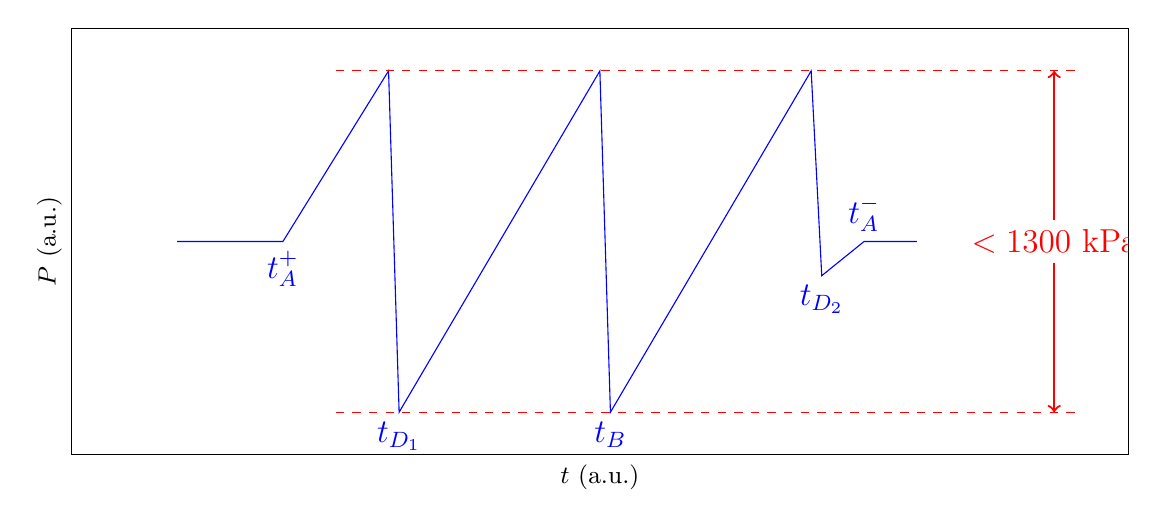
\begin{tikzpicture}
	\begin{axis}[
	width=15cm,
	height=7cm,
	xlabel=$t~(\mathrm{a.u.})$,
	ylabel=$P~(\mathrm{a.u.})$,
	xmin=0,
	xmax=1000,
	ymin=0,
	ymax=100,
	xtick=\empty,
	ytick=\empty,
	]
	\draw[blue] (10,50) -- (20,50) node[below] {\large $t_A^+$}-- (30,90) -- (31,10)  node[below] {\large $t_{D_1}$} -- (50,90) -- (51,10)  node[below] {\large $t_B$} -- (70,90) -- (71,42)  node[below] {\large $t_{D_2}$} -- (75,50)  node[above] {\large $t_A^-$} -- (80,50);
	\draw[dashed, red] (25,90) -- (95,90);
	\draw[dashed, red] (25,10) -- (95,10);
	\draw[->,thick, red] (93,55) -- (93,90);
	\node [red] at (93,50) {\large $<1300\pre$};
	\draw[->,thick, red] (93,45) -- (93,10) ;
	\end{axis}
	\end{tikzpicture}
	\caption{$\tau_A=\tau_B'$ 时,泵油、供油和喷油曲线的示意图}
	\label{sketch32}
\end{figure}
	
图 \ref{sketch32} 中,$t_A^+$ 开始油泵中有油泵出,直到 $t_A^-$才停止。在大部分时间油管内由于油泵泵油而压强增大;而在$t_{D_1}$附近减压阀开启压强下降,$t_B$附近喷油器喷油导致压强下降,$t_{D_2}$附近减压阀第二次开启。

$t_B$附近$1300\pre$的压降无可避免,我们要做的是调节$t_{D_1}$、$t_B$ 和 $t_{D_2}$及减压阀开启时长使得压强的波动范围在这个限度以内,并且最终管内压强能回到标准压强。

\subsubsection{减压阀受到限制情况:精确数值模拟}

我们沿用之前连续可调情况下的模拟程序,但是由于减压阀开启限制需要做一些调整:

\begin{enumerate}
	\item 定义布尔变量记录减压阀是否处于锁定的不可开启状态,并记录锁定的剩余时间,只有在减压阀未锁定时可以对其进行操作;
	\item 每当减压阀被关闭时,进入 $10\tim$ 的锁定时间;
	\item 更新油管总油量 $m_2$ 的代码区域需要做出较大改变。在减压阀锁定时直接按照无减压阀的情况更新 $m_2$;而在减压阀未锁定时需要根据此刻的时间和系统状态判断在示意图中哪个部分,以给减压阀正确的开关指令。
\end{enumerate}

最优方案给出的模拟结果如 \ref{discontinuumPt} 所示:

\begin{figure}[!ht]
	\centering
	\begin{tikzpicture}
	\begin{axis} [
		width = 10cm,
		height = 5cm,
		xlabel = {$t\tims$},
		ylabel = {$P_2-P_2^*\pres$},
		xmin = 0, 
		xmax = 300,
		%ymin = -2400,
		%ymax = 400,
		%ytick distance = 400,
	]
	\addplot table [
		x=t, 
		y=P_2, 
		mark=none, 
		smooth] {../3/t-P-2.dat};
	\end{axis}
	\end{tikzpicture}
	\caption{最优控制方案下,$P_2$ 与 $t$ 的关系}
	\label{discontinuumPt}
\end{figure}

在该条件下,最大偏差 $D_{\max}=636\pre$,极差 $E=1264\pre$ ,符合最优解的要求。计算得到此策略下均方根偏差为 $D=226\pre$,小于优化前(即第二题中)的四分之一,说明这一控制方案非常有效。

综上,我们的最终控制方案为:
\begin{itemize}
	\item 供油周期 $\tau_A=50\tim$;
	\item 喷油器 B 和 C 等间隔交替喷油;
	\item 相位时间 $\phi_B=10.35\tim$;
	\item 减压阀开启的时间为:每个 $\tau_B'=50\tim$ 内的 $[4.84\tim,6.29\tim]$ 和 $[17.43\tim, 18.75\tim]$。
\end{itemize}

\newpage
\section{模型的评价} % 优缺点、改进空间和范围
\subsection{问题1}
	该题中的模型所做的假设是管内压强是均匀的,在单向阀处燃油的流量根据题目中注2给出的公式计算。不考虑燃油的粘滞、涡流等复杂液体行为,也没有考虑燃油如何在油管内从一端流动至另一端。由于条件本身也是抽象化的,省略了很多细节,因此模型也简洁而清晰。当然也正是因为其简洁性,没有太多实际应用的价值。
\subsection{问题2}
	在问题2中,我们将问题1的高压泵和喷油器具象化了,考虑了他们的工作原理。
	这个模型同样认为所有封闭腔内的压强是均匀的,燃油是静止的,忽略了燃油的复杂流体性质。还有一个重要的假设是把喷油器内的流动看做是连续两次扩散过程。
	
	然而实际上喷油器处燃油的流动是非常复杂的,较精确的计算要使用混合多相流模型附加空穴模型\cite{模型评价1},本题这里的近似较为粗糙,这也是此模型最大的缺陷。
	
	但本模型的优点在于可修改性强,整个程序的核心物理量是管内燃油的质量 $m_2$,而油泵和喷油器对$m_2$的全部影响都体现为油管压强 $P_2$ 和时间 $t$ 的一个二元函数,这些函数互不干扰。因此后续改进可以是精确计算喷油器的流量模型,然后修改主程序中对应的函数即可,其它部分不受影响。
	
	本模型另一个优点是可拓展性强。比如说加一个喷油器或者加一个阀门,都只要更新$m_2$时加两个函数值即可,这也为问题3提供了方便。
\subsection{问题3}
	问题3的模型主要是通过减压阀的控制,实现了更加稳定的油管压强。
	该模型联系了实际。喷油器是给发动机供油的,而发动机转速在短时间内一般不会剧烈改变,因此模型假定了喷油器的喷油周期是恒定的。凸轮的角速度也很难快速地精确控制,因此假定了凸轮是匀速旋转。
	
	模型最终实现了非常好的稳压效果。若能连续调控减压阀,压强变化量几乎可以忽略。若考虑可能的实际情况,在减压阀调控受限时,通过一个周期内给定时间段仅开启两次减压阀也能实现不俗的效果。并且前文也证明了在这些假定下上述调控方案是最优的。
	
	从实际情况来看,更好地实现稳压需要更加精细的模型,例如要考虑针阀开启或关闭瞬间由于液体流动行为突然变化导致的压力波动。而实际情况中可能出现的影响压力的这些因素由于涉及到流体性质在本模型中无法计算。
  
	作为稳压装置,本油管的改进可以通过增加一个减压阀,允许更大的凸轮转速。也可以改变凸轮的形状,使油泵的泵油在一个周期内更加集中。

\newpage

\begin{thebibliography}{9}%宽度9
	\bibitem[1]{引言}
    白云.
    \newblock 高压共轨燃油系统循环喷油量波动特性研究\allowbreak[D].
    \newblock 哈尔滨工程大学,2017.

	\bibitem[2]{保持频率不变}
    仲志全,李华宇,尹琪.
    \newblock 发动机运行工况对机油耗影响的试验研究\allowbreak[J].
    \newblock 内燃机工程,2004(05):69-71.

	\bibitem[3]{减压阀}
    刘学龙,苏万华,战强.
    \newblock 高压油管对共轨系统性能影响的研究\allowbreak[J].
    \newblock 内燃机工程,2010,31(05):47-51+57.

	\bibitem[4]{锥形喷油嘴}
    陶希成.
    \newblock 柴油机锥形孔喷嘴内空穴流动及其对喷雾影响的试验研究\allowbreak[D].
    \newblock 江苏大学,2016.

    \bibitem[5]{模型评价1}
    崔慧峰,罗福强,董少锋,梁昱,周立迎.
    \newblock 柴油机渐缩形喷孔喷嘴流动特性研究\allowbreak[J].
    \newblock 农业机械学报,2013,44(11):19-25.

    \bibitem[6]{模型评价2}
    丁晓亮,张幽彤,苏海峰. 
    \newblock 压电式共轨系统喷油量压力波动修正策略研究\allowbreak[J].
    \newblock 北京理工大学学报. 2010(09)
\end{thebibliography}

\newpage

\begin{appendices}

\section{源代码}
\subsection{文件结构说明}
\begin{enumerate}
    \item 本文中全部代码使用 Python 3 编写,并使用 3.7.1 版本的解释器解释运行;
	\item \verb|data| 文件夹存放了以下内容:
	\begin{itemize}
		\item 题目中提供的数据:\verb|outline.raw| 为附件 1 中的凸轮边缘曲线,\verb|movement.raw| 为附件 2 中的针阀运动曲线,\verb|elasticity.raw| 为弹性模量与压力的关系;
		\item 处理原始数据生成可用数据的程序:\verb|process_outline.py| 处理凸轮边缘曲线生成高度与转角的关系并存放在 \verb|height.dat| 中,\verb|process_elasticity.py| 处理弹性模量生成压力与密度的关系并存放在 \verb|density.dat| 中;
		\item 函数库程序:\verb|lib.py| 存放了问题 1 至 3 所共用的一系列函数。
	\end{itemize}
    \item \verb|1| 文件夹存放了以下内容:
	\begin{itemize}
		\item 基于稳压近似的估算程序:\verb|analysis.py|,结果输出到屏幕上;
		\item 系统 1 的数值模拟程序:\verb|simulation1.py|,结果保存到 \verb|P-t.dat|、\newline \verb|D-tauA20/40/60/80/100.dat|、\verb|tau-N.dat|;
		\item 系统 1 压力调整的模拟程序:\verb|adjustment.py|,结果保存到 \newline \verb|adjustment_in_2000/5000/10000.dat|。
	\end{itemize}
    \item \verb|2| 文件夹存放了以下内容:
	\begin{itemize}
		\item 系统 2 的数值模拟程序:\verb|simulation2.py|,结果保存到 \verb|P-t.dat|、\verb|D-omega.dat|、\verb|m1-t.dat|、\verb|QA-t.dat|。
	\end{itemize}
    \item \verb|3| 文件夹存放了以下内容:
	\begin{itemize}
		\item 在连续情况下,系统 3 的数值模拟程序:\verb|simulation3_1.py|,结果保存到 \newline \verb|t-P-1.dat|;
		\item 在非连续情况下,系统 3 的数值模拟程序:\verb|simulation3_2.py|,结果保存到 \newline \verb|t-P-2.dat|。
	\end{itemize}
    % \item \verb|3-非连续| 文件夹存放了以下内容:
	% \begin{itemize}
	% 	\item 在非连续情况下,系统 3 的数值模拟程序:\verb|simulation4.py|,结果保存到 \verb|simulation4.dat|。
	% \end{itemize}
\end{enumerate}
\subsection{函数库及预处理源代码}

\lstinputlisting[
style       =   Python,
caption     =   {将弹性模量处理为密度数据}
]{../data/process_elasticity.py}

\lstinputlisting[
style       =   Python,
caption     =   {将凸轮轮廓处理为高度数据}
]{../data/process_outline.py}

\lstinputlisting[
style       =   Python,
caption     =   {函数库}
]{../data/lib.py}

\subsection{第一题源代码}

\lstinputlisting[
style       =   Python,
caption     =   {系统 1 的解析计算}
]{../1/analysis.py}

\lstinputlisting[
style       =   Python,
caption     =   {系统 1 的数值模拟}
]{../1/simulation.py}

\lstinputlisting[
style       =   Python,
caption     =   {系统 1 的压力调整模拟}
]{../1/adjustment.py}

\subsection{第二题源代码}

\lstinputlisting[
style       =   Python,
caption     =   {系统 2 的数值模拟}
]{../2/simulation2.py}

\subsection{第三题源代码}

\lstinputlisting[
style       =   Python,
caption     =   {系统 3 的数值模拟,连续情况}
]{../3/simulation3_1.py}

\lstinputlisting[
style       =   Python,
caption     =   {系统 3 的数值模拟,非连续情况}
]{../3/simulation3_2.py}

\end{appendices}
\end{document} 